\documentclass[12pt, a4paper]{ctexart} % 直接使用中文文档类

% ---------- 页面设置 ----------
\usepackage{algorithm}      % 算法环境
\usepackage{algorithmic}    % 算法伪代码
\usepackage{amsmath}        % 数学公式支持
\usepackage{geometry}
\usepackage{indentfirst}   % 让首段也缩进
\usepackage{graphicx}
\usepackage{amsfonts} % 或者使用 \usepackage{amssymb}////为了使用黑体字公式
\usepackage{booktabs}%三线表格式

\setlength{\parindent}{2em} % 缩进2字符(1em≈1汉字宽度)
\geometry{left=3cm, right=2.5cm, top=2.5cm, bottom=2.5cm}

% ---------- 字体配置 ----------
\setmainfont{Times New Roman}          % 设置西文字体

% ---------- 段落格式 ----------
\linespread{1.5}                      % 1.5倍行距
\setlength{\parindent}{2em}           % 首行缩进

% ---------- 标题格式 ----------
\usepackage{titlesec}
\titleformat{\section}{\Large\bfseries\heiti}{\thesection}{1em}{}
\titleformat{\subsection}{\large\bfseries\heiti}{\thesubsection}{1em}{}

% ---------- 文档信息 ----------
\title{“我为什么要相信你?”解释任何分类器的预测}
\author{译者Tinkle}
\date{\today}

\begin{document}
\maketitle{}
% ---------- 摘要页 ----------
\begin{abstract}
    尽管被广泛的采用,机器学习模型大多是黑匣子。然而,了解预测背后的原因对于评估信任非常重要,如果一个人计划根据预测采取行动,或者在选择是否部署新模型时,这一点至关重要。这种理解还提供了对模型的见解,可用于将不可信的模型或预测转换为可信的模型或预测。
    
    在这项工作中,我们提出了 LIME,这是一种新颖的解释技术,通过围绕预测在本地学习可解释模型,以可解释和忠实的方式解释任何分类器的预测。我们还提出了一种解释模型的方法,通过以非冗余的方式呈现具有代表性的单个预测及其解释,将任务构建为子模优化问题。我们通过解释文本(例如随机森林)和图像分类(例如神经网络)的不同模型来展示这些方法的灵活性。我们通过模拟和人类受试者的新颖实验来展示解释在各种需要信任的场景中的效用:决定是否应该相信预测、在模型之间进行选择、改进不可信的分类器以及确定为什么不应该信任分类器。
\end{abstract}

% ---------- 正文部分 ----------
\section{引言}
机器学习是许多最新科学和技术进步的核心。不幸的是,人类的重要作用是该领域经常被忽视的一个方面。无论人类是直接使用机器学习分类器作为工具,还是在其他产品中部署模型,一个至关重要的问题仍然存在:如果用户不信任模型或预测,他们就不会使用它。区分信任的两种不同(但相关)定义很重要:(1) 信任预测,即用户是否足够信任单个预测以根据它采取一些行动,以及 (2) 信任模型,即用户是否相信模型在部署后会以合理的方式运行。

两者都收到人类对模型行为的理解程度,而不是将其视为黑匣子。当模型用于决策时,确定对单个预测的信任度是一个重要问题。例如,当使用机器学习进行医疗诊断 [6] 或恐怖主义侦查时,不能盲目相信地进行预测,因为后果可能是灾难性的。

除了信任单个预测之外,还需要在“野外”部署模型之前将其作为一个整体进行评估。要做出此决定,用户需要确信该模型将根据感兴趣的指标在实际数据上表现良好。目前,模型使用可用验证数据集上的准确率指标进行评估。但是,实际数据通常存在显著差异,此外,评估指标可能并不表示产品的目标。除了此类指标之外,检查单个预测及其解释也是一种有价值的解决方案。在这种情况下,通过建议要检查的实例来帮助用户非常重要,尤其是对于大型数据集。

在本文中,我们建议为单个预测提供解释作为 “信任预测 ”问题的解决方案,并选择多个这样的预测 (和解释) 作为 “信任模型 ”问题的解决方案。我们的主要贡献总结如下。

LIME,一种可以通过使用可解释模型进行局部近似来忠实地解释任何分类器或回归器的预测的算法。

SP-LIME,一种通过子模优化选择一组具有代表性实例并附有解释来解决“信任模型”问题的方法。

对模拟和人类受试者进行综合评估,我们衡量解释对信任和相关任务的影响。在我们的实验中,使用 LIME 的非专家能够从一对分类器中选择哪个分类器在现实世界中泛化得更好。此外,通过使用 LIME 进行特征工程,他们能够大大改进在 20 个新闻组上训练的不可信分类器。我们还展示了了解神经网络对图像的预测如何帮助从业者了解何时以及为什么不应该信任模型。

\section{解释的理由}
“解释预测”是指呈现文本或视觉工件,这些工件提供了对实例组件(例如文本中的单词、图像中的补丁)与模型预测之间关系的定性理解。我们认为,解释预测是让人类信任并有效使用机器学习的一个重要方面,前提是解释要忠实、易懂。

\begin{figure}[h]
    \centering
    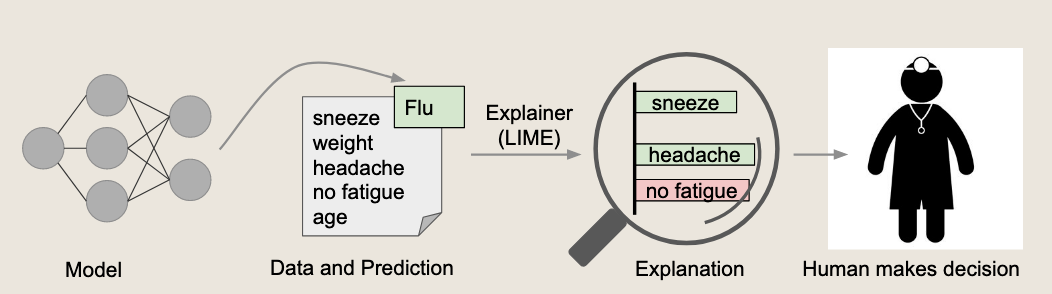
\includegraphics[width=0.6\textwidth]{img/img_1.png}
    \caption{解释单个预测。模型预测患者患有流感,而 LIME 会突出显示患者病史中导致预测的症状。打喷嚏和头痛被描绘成有助于 “流感 ”预测,而 “没有疲劳 ”则是反对它的证据。有了这些,医生可以就是否信任模型的预测做出明智的决定。}
    \label{fig:img_1}
\end{figure}

解释单个预测的过程如图 1 所示。很明显,如果提供可理解的解释,医生在模型的帮助下更有能力做出决定。在这种情况下,解释是一小部分症状,这些症状具有相对权重的症状,这些症状要么有助于预测(绿色),要么是反对预测的证据(红色)。人类通常具有有关应用程序域的先验知识,如果他们了解预测背后的原因,他们可以使用这些知识来接受(信任)或拒绝预测。例如,据观察,提供解释可以提高对电影推荐和其他自动化系统。

每个机器学习应用程序还需要对模型进行一定程度的总体信任。分类模型的开发和评估通常包括收集带注释的数据,其中保留的子集用于自动评估。尽管这对许多应用程序来说是一个有用的管道,但对验证数据的评估可能与“在野外”的性能不对应,因为从业者经常高估其模型的准确性 [20],因此信任不能仅仅依赖它。查看示例提供了一种评估模型中的真值的方法,尤其是在解释示例的情况下。因此,我们建议解释模型的几个代表性个体预测,作为提供全局理解的一种方式。

模型或其评估可能以多种方式出错。例如,数据泄漏被定义为信号无意中泄漏到训练(和验证)数据中,而这些数据在部署时不会出现 [14],这可能会提高准确性。Kaufman等[14]引用了一个具有挑战性的例子,即发现患者ID与训练和验证数据中的目标类别高度相关。仅通过观察预测和原始数据来识别这个问题将非常具有挑战性,但如果提供如图 1 中的解释,则要容易得多,因为患者 ID 将被列为预测的解释。另一个特别难以检测的问题是数据集偏移 [5],其中训练数据与测试数据不同(我们稍后会在著名的 20 个新闻组数据集中举一个例子)。解释给出的见解对于确定必须采取哪些措施来将不可信的模型转换为可信的模型特别有用,例如,删除泄露的数据或更改训练数据以避免数据集偏移。

\begin{figure}[h]
    \centering
    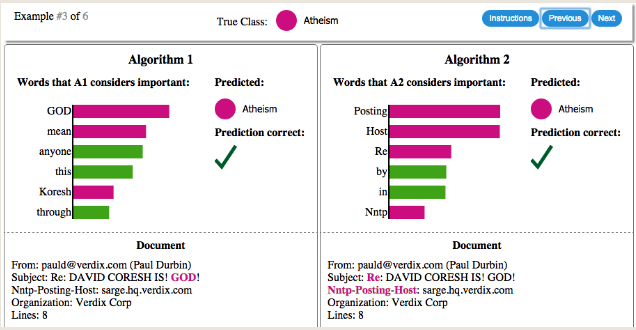
\includegraphics[width=0.6\textwidth]{img/img_2.png}
    \caption{解释竞争分类器的个体预测,试图确定文档是关于 “基督教” 还是 “无神论” 的。条形图表示对最相关单词的重视程度,在文本中也突出显示。颜色表示该词属于哪个类别(绿色代表 “Christianity”,洋红色代表 “Atheism”)}
    \label{fig:img_2}
\end{figure}
机器学习从业者通常必须从许多备选方案中选择一个模型,这需要他们评估两个或多个模型之间的相对信任度。在图2我们展示了如何使用单个预测解释在模型之间进行选择,以及准确性。在这种情况下,在验证集上具有较高准确性的算法实际上要差得多,当提供解释时(同样,由于人类的先验知识),这一事实很容易看到,否则就很难了。此外,我们可以计算和优化的指标(例如准确性)与实际感兴趣的指标(例如用户参与度和留存率)之间经常存在不匹配。虽然我们可能无法衡量这些指标,但我们了解某些模型行为如何影响它们。因此,从业者可能希望选择一种不太准确的内容推荐模型,该模型不高度重视与 “点击诱饵” 文章相关的特征(这可能会损害用户留存),即使利用这些特征可以提高模型在交叉验证中的准确性。我们注意到,如果一种方法可以为任何模型生成解释,那么在这些(和其他)场景中,解释特别有用,以便可以比较各种模型。

\subsection{解释器所需的特性}
现在,我们从解释方法中概述了一些所需的特征。解释的一个基本标准是它们必须是可解释的,即在输入变量和响应之间提供定性理解。我们注意到,可解释性必须考虑到用户的局限性。因此,线性模型 [24]、梯度向量 [2] 或加法模型 [6] 可能是可解释的,也可能是不可解释的。例如,如果成百上千个特征对预测有重大贡献,那么期望任何用户都能理解做出预测的原因也是不合理的,即使可以检查单个权重也是如此。这一要求进一步意味着解释应该易于理解,而模型使用的特征不一定如此,因此解释中的“输入变量”可能需要与特征不同。最后,我们注意到可解释性的概念也取决于目标受众。机器学习从业者可能能够解释小型贝叶斯网络,但外行人可能更愿意使用少量加权特征作为解释。

另一个基本标准是本地保真度。尽管除非是模型本身的完整描述,否则解释通常不可能完全忠实,但要使解释有意义,它至少必须忠实于局部,即它必须与模型在被预测实例附近的行为相对应。我们注意到,局部保真度并不意味着全局保真度:全局重要的特征在本地上下文中可能不重要,反之亦然。虽然全局保真度意味着局部保真度,但确定可解释的全局忠实解释仍然是复杂模型面临的挑战。

虽然有些模型本质上是可解释的 [6, 17, 26, 27],但解释者应该能够解释任何模型,因此与模型无关(即将原始模型视为黑匣子)。除了许多最先进的分类器目前不可解释之外,这也为解释未来的分类器提供了灵活性。

除了解释预测之外,提供全局视角对于确定对模型的信任也很重要。如前所述,准确性通常不是评估模型的合适指标,因此我们想解释一下这个模型。在对单个预测的解释的基础上,我们选择了一些解释来呈现给用户,以便它们能够代表模型。

\section{与模型无关的本地可解释性解释}
我们现在提出与模型无关的本地可解释性解释 Local Interpretable Model-agnostic Explanations (LIME)。LIME 的总体目标是在局部忠实于分类器的可解释表示上确定一个可解释模型。
\subsection{可解释的数据表示}
在我们介绍解释系统之前,区分特征和可解释数据表示是很重要的。如前所述,可解释的解释需要使用人类可以理解的表示形式,而不管模型使用的实际特征如何。例如,文本分类的可能可解释表示是指示单词存在或不存在的二进制向量,即使分类器可能使用更复杂(和难以理解)的特征,例如单词嵌入。同样,对于图像分类,可解释表示可以是二进制向量,表示“存在”或“不存在”相似像素的连续块(超级像素),而分类器可以将图像表示为每个像素具有三个颜色通道的张量。我们将$x\in\mathbb{R}^d$表示为所解释实例的原始表示,我们使用 $x^{\prime}\in\{0,1\}^{d^{\prime}}$ 来表示其可解释表示的二进制向量。
\subsection{保真度-可解释性权衡}
正式地,我们将解释定义为一个模型 \( g \in G \),其中 \( G \) 是一类潜在可解释的模型,例如线性模型、决策树或规则列表,即 \( g \in G \) 可以通过视觉或文本方式清晰地呈现给用户。\( g \) 的定义域为 \( \{0,1\}^{d'} \),即 \( g \) 通过解释性组件的存在/缺失进行作用。由于并非所有 \( g \in G \) 都足够简单到可以被解释,我们用 \( \Omega(g) \) 来衡量解释 \( g \in G \) 的复杂性(相对于可解释性)。例如,对于决策树来说,\( \Omega(g) \) 可以表示树的深度,而对于线性模型来说,\( \Omega(g) \) 可以表示非零权重的数量。

设被解释的模型表示为 \( f: \mathbb{R}^d \to \mathbb{R} \)。在分类任务中,\( f(x) \) 代表 \( x \) 属于某一类别的概率(或二元指示器)\(^1\)。此外,我们使用 \( \pi_x(z) \) 作为度量 \( z \) 到 \( x \) 之间的接近程度,从而定义 \( x \) 周围的局部区域。最后,定义 \( \mathcal{L}(f, g, \pi_x) \) 作为衡量 \( g \) 在 \( \pi_x \) 所定义的局部区域内对 \( f \) 近似程度的不准确性。

为了确保 \textbf{可解释性} 和 \textbf{局部保真性},我们必须最小化 \( \mathcal{L}(f, g, \pi_x) \) ,同时保证 \( \Omega(g) \) 低到足够可被人类理解的程度。LIME 生成的解释可由如下公式给出:

\[
\xi(x) = \arg\min_{g \in G} \mathcal{L}(f, g, \pi_x) + \Omega(g)
\]

该公式可用于不同的解释模型族 \( G \)、保真性度量函数 \( \mathcal{L} \) 和复杂性度量 \( \Omega \)。本文重点研究稀疏线性模型作为解释,并通过扰动进行搜索。
\subsection{局部探索的采样}
我们希望最小化局部感知损失 \( \mathcal{L}(f, g, \pi_x) \),而不对 \( f \) 作任何假设,因为我们希望解释器具有\textbf{模型无关性(model-agnostic)}。因此,为了学习 \( f \) 在可解释输入变化时的局部行为,我们通过抽样近似 \( \mathcal{L}(f, g, \pi_x) \),并使用 \( \pi_x \) 进行加权。我们通过对 \( x' \) 的非零元素进行均匀随机采样(采样数量也是均匀分布的)来生成 \( x' \) 周围的样本。

给定一个扰动后的样本 \( z' \in \{0,1\}^{d'} \)(其中包含 \( x' \) 的部分非零元素),我们恢复其在原始表示中的样本 \( z \in \mathbb{R}^d \),并计算 \( f(z) \),将其作为解释模型的\textbf{标签}。给定这样一个包含扰动样本及其对应标签的数据集 \( \mathcal{Z} \),我们优化公式 (1) 以获得解释 \( \xi(x) \)。

LIME 的基本直觉在图 3 中进行了展示,其中我们在 \( x \) 附近(由于 \( \pi_x \) 具有较高权重)和远离 \( x \) 的区域(由于 \( \pi_x \) 具有较低权重)同时进行采样。尽管原始模型可能过于复杂,无法在全局范围内解释,但 LIME 生成的解释在局部范围内是\textbf{忠实}的(在本例中是线性的),其中局部性由 \( \pi_x \) 捕获。

值得注意的是,我们的方法对采样噪声具有较强的鲁棒性,因为在公式 (1) 中,样本是通过 \( \pi_x \) 进行加权的。接下来,我们将给出该通用框架的具体实例。
\subsection{稀疏线性解释}
对于本文的其余部分,我们令 \( G \) 为线性模型类,使得 \( g(z') = w_g \cdot z' \)。我们使用局部加权平方损失作为 \( \mathcal{L} \),其定义如公式 (2) 所示,其中我们令
\[
\pi_x(z) = \exp(-D(x, z)^2 / \sigma^2)
\]
为某种指数核函数。距离函数 D(例如,文本的余弦距离,图像的 L2 距离)的宽度为 σ。

\[\mathcal{L}(f, g, \pi_x) = \sum_{z, z' \in \mathcal{Z}} \pi_x(z) \left( f(z) - g(z') \right)^2 \quad (2)\]

\begin{figure}[h]
    \centering
    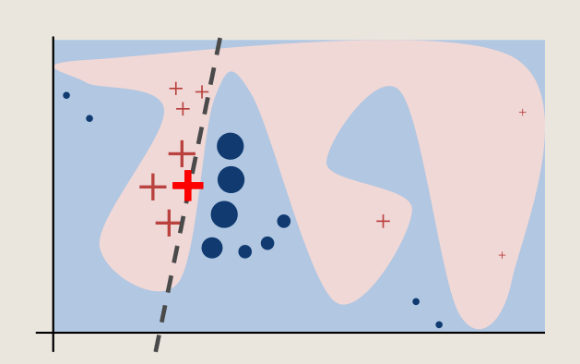
\includegraphics[width=0.6\textwidth]{img/img_3.png}
    \caption{玩具示例,用于展示 LIME 的直觉。黑盒模型的复杂决策函数 f(LIME 未知)由蓝色/粉红色背景表示,线性模型无法很好地近似。粗体红叉是正在解释的实例。LIME 对实例进行采样,使用 f 获取预测,并根据与所解释的实例的接近程度(此处用 size 表示)对它们进行加权。虚线是本地(但不是全局)忠实的学习解释。}
    \label{fig:img_3}
\end{figure}

对于文本分类,我们通过将可解释表示设置为词袋模型,并限制词的数量为\(K\),即当\(\|w_g\|_0 > K\)时,\(\Omega(g) = \infty\),来确保解释是可解释的。\(K\)可以调整为用户能够处理的最大值,或者我们可以为不同的实例设置不同的\(K\)值。在本文中,我们使用一个常数\(K\)值,将探索不同\(K\)值的工作留待未来研究。我们对图像分类使用相同的\(\Omega\),使用“超像素”(通过任何标准算法计算)代替词,使得图像的可解释表示是一个二进制向量,其中1表示原始超像素,0表示灰度化的超像素。这种特定的\(\Omega\)选择使得直接求解方程(1)变得不可行,但我们通过首先使用Lasso选择\(K\)个特征(使用正则化路径[9]),然后通过最小二乘法学习权重(我们在算法1中称为K-LASSO)来近似它。由于算法1为单个预测生成解释,其复杂度不依赖于数据集的大小,而是依赖于计算\(f(x)\)的时间和样本数量\(N\)。在实践中,使用scikit-learn(http://scikit-learn.org)在一台笔记本电脑上解释具有1000棵树的随机森林,当\(N=5000\)时,无需任何优化(如使用GPU或并行化),耗时不到3秒。解释Inception网络[25]的每个图像分类预测大约需要10分钟。

\begin{algorithm}
    \caption{使用LIME的稀疏线性解释}
    \begin{algorithmic}[1]
    \REQUIRE 分类器 \(f\),样本数量 \(N\)
    \REQUIRE 实例 \(x\) 及其可解释版本 \(x'\)
    \REQUIRE 相似性核 \(\pi_x\),解释长度 \(K\)
    \STATE \(\mathcal{Z} \leftarrow \{\}\)
    \FOR{\(i \in \{1, 2, 3, ..., N\}\)}
        \STATE \(z'_i \leftarrow\) 在 \(x'\) 周围采样
        \STATE\(\mathcal{Z} \leftarrow \mathcal{Z} \cup \langle z'_i, f(z_i), \pi_x(z_i) \rangle\)
    \ENDFOR
    \STATE \(w \leftarrow\) K-Lasso(\(\mathcal{Z}\), \(K\)),其中 \(z'_i\) 为特征,\(f(z)\) 为目标
    \RETURN \(w\)
    \end{algorithmic}
\end{algorithm}
    
任何可解释表示和\(G\)的选择都会有一些固有的缺点。首先,尽管底层模型可以被视为黑盒,但某些可解释表示可能不足以解释某些行为。例如,一个预测棕褐色调图像为“复古”的模型不能通过超像素的存在或缺失来解释。其次,我们选择的\(G\)(稀疏线性模型)意味着,如果底层模型在预测的局部区域内高度非线性,可能没有一个忠实的解释。然而,我们可以在\(\mathcal{Z}\)上估计解释的忠实度,并将这些信息呈现给用户。这种忠实度估计也可以用于从多个可解释模型类中选择合适的解释族,从而适应给定的数据集和分类器。我们将这种探索留待未来研究,因为在我们的实验中,线性解释对多个黑盒模型效果很好。

\subsection{示例 1:使用 SVM 进行文本分类}
在图2(右侧),我解释了一个使用RBF核的支持向量机(SVM)的预测,该SVM训练在单个词上,用于区分“基督教”和“无神论”(使用20个新闻组数据集的一个子集)。尽管这个分类器达到了94\%的保留测试集准确率,但对一个实例的解释显示,预测是基于相当随意的原因做出的(“Posting”、“Host”和“Re”这些词与基督教或无神论没有任何关联)。词“Posting”出现在训练集中22\%的示例中,其中99\%属于“无神论”类别。即使移除了头部信息,原始新闻组中频繁发帖者的专有名词仍被分类器选中,这也不会泛化。
在从解释中获得这些见解后,很明显,这个数据集存在严重的问题(这些问题仅通过研究原始数据或预测是无法发现的),并且这个分类器或保留测试集评估不能被信任。同时,也很清楚问题所在,以及可以采取的步骤来解决这些问题,训练一个更值得信赖的分类器。

\subsection{示例 2:图像的深度网络}
\begin{figure}[h]
    \centering
    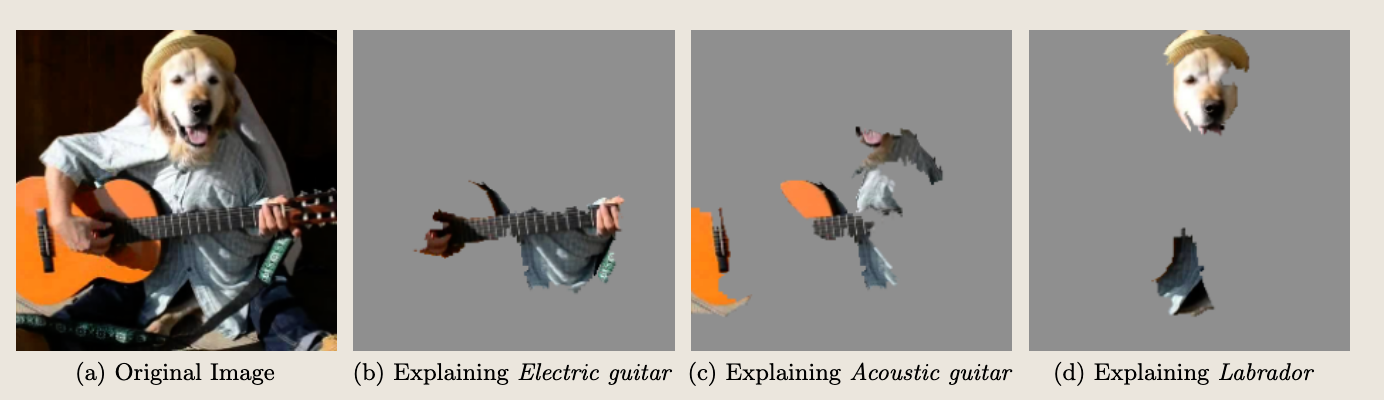
\includegraphics[width=0.8\textwidth]{img/img_4.png}
    \caption{解释由谷歌的Inception神经网络做出的图像分类预测。预测的前三个类别分别是“电吉他”(概率0.32)、“原声吉他”(概率0.24)和“拉布拉多犬”(概率0.21)。}
\end{figure}
使用稀疏线性解释来解释图像分类器时,人们可能希望仅突出显示对特定类别具有正权重的超像素,因为它们可以直观地说明模型为何认为该类别可能存在。我们以这种方式解释了Google预训练的Inception神经网络[25]对任意图像(图4a)的预测。图4b、4c、4d展示了前3个预测类别的超像素解释(图像的其余部分被灰化),其中K=10。神经网络对每个类别的关注点对人类来说非常自然——特别是图4b提供了为什么预测声学吉他为电吉他的见解:因为琴颈。这种解释增强了对分类器的信任(即使预测的类别是错误的),因为它表明模型并非以不合理的方式行事。

\section{用于解释模型的子模拾取}
虽然对单个预测的解释为用户提供了对分类器可靠性的一定理解,但这不足以评估和判断整个模型的可信度。我们建议通过解释一组个体实例来提供对模型的全局理解。这种方法仍然是模型无关的,并且可以补充诸如保留集准确率等统计方法。

尽管多个实例的解释可能具有洞察力,但这些实例需要谨慎选择,因为用户可能没有时间检查大量的解释。我们用预算 \(B\) 来表示人类的时间/耐心,即他们愿意查看的解释数量,以便理解一个模型。给定一组实例 \(X\)(\(|X| = n\)),我们定义“选择步骤”(pick step)为选择 \(B\) 个实例供用户检查的任务。

选择步骤并不依赖于解释的存在——像Modeltracker这样的工具的主要目的是帮助用户自己选择实例,并检查原始数据和预测。然而,由于查看原始数据不足以理解预测并获得洞察,选择步骤应考虑每个预测的解释。此外,这种方法应选择一组多样化、有代表性的解释来展示给用户,即非冗余的解释,代表模型的全局行为。

\begin{figure}[h]
    \centering
    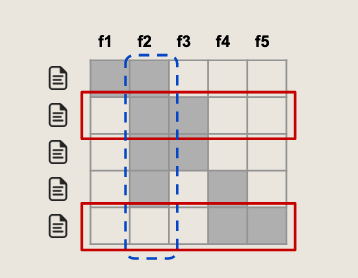
\includegraphics[width=0.6\textwidth]{img/img_5.png}
    \caption{玩具示例 \(\mathcal{W}\)。行表示实例(文档),列表示特征(词)。特征 \(f2\)(点状蓝色)具有最高的重要性。第2行和第5行(红色)将被选择过程选中,覆盖了除 \(f1\) 之外的所有特征。}
    \label{fig:img_5}
\end{figure}
    
给定一组实例 \(X\)(\(|X| = n\)),我们构建一个 \(n \times d'\) 的解释矩阵 \(\mathcal{W}\),表示每个实例的可解释组件的局部重要性。当使用线性模型作为解释时,对于实例 \(x_i\) 和解释 \(g_i = \xi(x_i)\),我们设置 \(\mathcal{W}_{ij} = |w_{g_i,j}|\)。此外,对于 \(\mathcal{W}\) 中的每个组件(列)\(j\),我们让 \(I_j\) 表示该组件在解释空间中的全局重要性。直观上,我们希望 \(I\) 使得解释许多不同实例的特征具有更高的重要性分数。在图5中,我们展示了一个玩具示例 \(\mathcal{W}\),其中 \(n = d' = 5\),\(\mathcal{W}\) 是二进制的(为了简单起见)。重要性函数 \(I\) 应该给特征 \(f2\) 赋予比特征 \(f1\) 更高的分数,即 \(I_2 > I_1\),因为特征 \(f2\) 被用来解释更多的实例。具体到文本应用中,我们设置 \(I_j = \sqrt{\sum_{i=1}^{n} \mathcal{W}_{ij}}\)。对于图像,\(I\) 必须测量一些可以在不同图像的超像素之间进行比较的东西。
\begin{algorithm}
    \caption{子模选择(SP)算法}
    \begin{algorithmic}[1]
    \REQUIRE 实例 \(X\),预算 \(B\)
    \FORALL{\(x_i \in X\)}
        \STATE \(\mathcal{W}_i \leftarrow \text{explain}(x_i, x_i')\) \COMMENT{使用算法1}
    \ENDFOR
    \FOR{\(j \in \{1, \ldots, d'\}\)}
        \STATE\(I_j \leftarrow \sqrt{\sum_{i=1}^{n} |\mathcal{W}_{ij}|}\) \COMMENT{计算特征重要性}
    \ENDFOR
    \STATE \(V \leftarrow \{\}\)
    \WHILE{\(|V| < B\)}
        \STATE\(V \leftarrow V \cup \arg\max_i c(V \cup \{i\}, \mathcal{W}, I)\) \COMMENT{对公式(4)进行贪心优化}
    \ENDWHILE
    \RETURN \(V\)
    \end{algorithmic}
    \end{algorithm}
虽然我们希望选择能够覆盖重要组件的实例,但展示给用户的解释集在组件上不应冗余,即避免选择具有相似解释的实例。在图5中,选择第二行后,第三行没有增加任何价值,因为用户已经看到了特征 \(f2\) 和 \(f3\)——而最后一行则向用户展示了全新的特征。选择第二行和最后一行几乎覆盖了所有特征。我们在公式(3)中形式化了这种非冗余覆盖的直觉,其中我们定义覆盖为集合函数 \(c\),给定 \(\mathcal{W}\) 和 \(I\),计算至少在一个实例集中出现的特征的总重要性。

覆盖函数定义为:
\[
c(V, \mathcal{W}, I) = \sum_{j=1}^{d'} \mathbb{I}\left[\exists i \in V : \mathcal{W}_{ij} > 0\right] I_j \quad (3)
\]

选择问题定义在公式(4)中,目标是找到一个集合 \(V\),使得 \(|V| \leq B\),并且覆盖度最高。
\[
\text{Pick}(\mathcal{W}, I) = \arg\max_{V, |V| \leq B} c(V, \mathcal{W}, I) \quad (4)
\]

公式(4)中的问题是最大化一个加权覆盖函数,这是一个NP难问题 [10]。设 \(c(V \cup \{i\}, \mathcal{W}, I) - c(V, \mathcal{W}, I)\) 为将实例 \(i\) 添加到集合 \(V\) 中的边际覆盖增益。由于子模性,一个贪心算法,通过迭代地将具有最高边际覆盖增益的实例添加到解中,可以提供一个常数因子的近似保证,即最优解的 \(1 - 1/e\) [15]。我们在算法2中概述了这个近似算法,并称之为子模选择。

\section{模拟用户实验}
在本节中,我们提供了模拟用户实验,以评估解释在信任相关任务中的效用。特别是,我们解决了以下问题:(1) 解释是否忠实于模型,(2) 解释能否帮助用户确定对预测的信任度,以及 (3) 解释是否有助于评估整个模型。用于复制实验的代码和数据可在 https://github.com/marcotcr/lime-experiments 上获得。
\subsection{实验设置}
我们使用了两个情感分析数据集(书籍和DVD,各有2000个实例),任务是将产品评论分类为正面或负面 [4]。我们训练了决策树(DT)、带有L2正则化的逻辑回归(LR)、最近邻(NN)和支持向量机(SVM),所有这些都使用词袋模型作为特征。我们还包括了使用平均word2vec嵌入 [19] 训练的随机森林(1000棵树)(RF),这是一种没有LIME这样的技术就无法解释的模型。除非另有说明,我们使用scikit-learn的实现和默认参数。我们将每个数据集分为训练集(1600个实例)和测试集(400个实例)。
为了解释单个预测,我们将我们提出的方法(LIME)与Parzen [2] 进行了比较,Parzen是一种通过Parzen窗口全局近似黑盒分类器的方法,并通过取预测概率函数的梯度来解释单个预测。对于Parzen,我们取绝对梯度最高的K个特征作为解释。我们使用交叉验证设置Parzen和LIME的超参数,并设置N = 15,000。我们还将我们的方法与一种贪婪方法(类似于Martens和Provost [18])进行了比较,该方法贪婪地移除对预测类别贡献最大的特征,直到预测类别发生变化(或达到K个特征的最大值),以及一种随机方法,该方法随机选择K个特征作为解释。在我们的实验中,我们将K设置为10。
对于应用选择过程的实验,我们要么进行随机选择(随机选择,RP),要么进行第4节中描述的过程(子模选择,SP)。我们通过在解释器组合前加上RP或SP作为前缀来引用它们。

\subsection{解释是否忠实于模型?}
\begin{figure}[htbp]
    \centering
    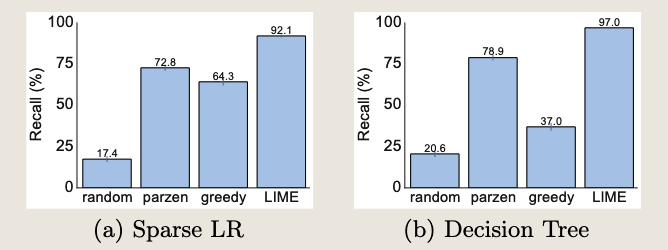
\includegraphics[width=0.6\textwidth]{img/img_6.png}
    \caption{图书数据集上两种可解释分类器的真正重要特征的回收率。。}
    \label{fig:img_6}
\end{figure}
\begin{figure}[h]
    \centering
    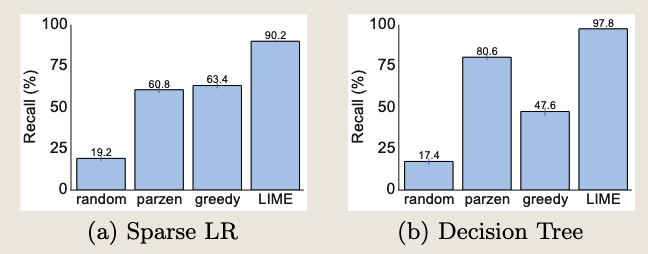
\includegraphics[width=0.6\textwidth]{img/img_7.png}
    \caption{DVD 数据集上两种可解释分类器的真正重要特征的回收率。}
    \label{fig:img_7}
\end{figure}
我们衡量本身可解释的分类器(稀疏 Logistic 回归和决策树)。特别是,我们训练两个分类器,使它们用于任何实例的最大特征数为 10,因此我们知道这些模型认为重要的黄金特征集。对于测试集上的每个预测,我们生成解释并计算解释恢复的这些黄金特征的比例。我们报告了图 6 和图 7 中所有测试实例的平均值。我们观察到,贪婪方法在 logistic 回归上与 parzen 相当,但在决策树上要差得多,因为一次更改单个特征通常不会对预测产生影响。parzen 的总体召回率很低,可能是由于难以近似原始高维分类器。LIME 始终为两个数据集上的两个分类器提供 90\% 的召回率>这表明 LIME 解释忠实于模型。

\subsection{我应该相信这个预测吗?}
为了模拟对单个预测的信任,我们首先随机选择 25\% 的特征为 “不可信”,并假设用户可以识别并且不想信任这些特征(例如 20 个新闻组中的标题、泄露的数据等)。因此,我们开发了 oracle “trustworthiness”,方法是将来自黑盒分类器的测试集预测标记为 “untrustity” (如果从实例中删除不可信特征时预测发生变化),否则标记为 “trustworthy”。为了模拟用户,我们假设用户认为 LIME 和 parzen 解释的预测不可信,如果当去除解释中出现的所有不可信特征时,线性近似的预测发生变化(模拟的人类“打折”了不可信特征的效果)。对于贪婪和随机,如果解释中存在任何不可信的特征,则预测不可信,因为这些方法不提供每个特征对预测的贡献的概念。因此,对于每个测试集预测,我们可以使用每种解释方法评估模拟用户是否信任它,并将其与可信度预言机进行比较。

\begin{table}[htbp]
    \centering
    \caption{分类器和数据集集合上不同解释器的平均可信度 F1。.}
    \begin{tabular}{|l|c|c|c|c|c|c|c|c|}
    \hline
     & \multicolumn{4}{c|}{Books} & \multicolumn{4}{c|}{DVDs} \\
    \hline
     & LR & NN & RF & SVM & LR & NN & RF & SVM \\
    \hline
    Random & 14.6 & 14.8 & 14.7 & 14.7 & 14.2 & 14.3 & 14.5 & 14.4 \\
    \hline
    Parzen & 84.0 & 87.6 & 94.3 & 92.3 & 87.0 & 81.7 & 94.2 & 87.3 \\
    \hline
    Greedy & 53.7 & 47.4 & 45.0 & 53.3 & 52.4 & 58.1 & 46.6 & 55.1 \\
    \hline
    LIME & 96.6 & 94.5 & 96.2 & 96.7 & 96.6 & 91.8 & 96.1 & 95.6 \\
    \hline
    \end{tabular}
\end{table}

\begin{figure}[h]
    \centering
    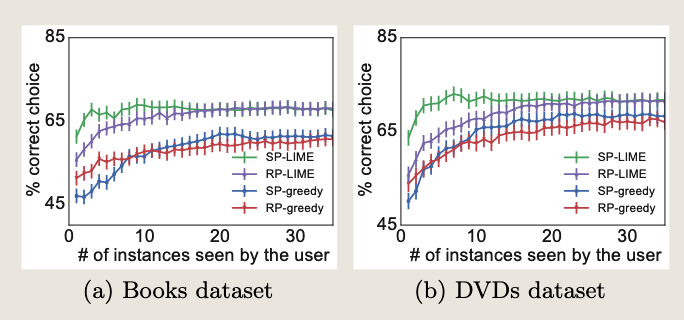
\includegraphics[width=0.6\textwidth]{img/img_8.png}
    \caption{在两个分类器之间进行选择,因为向模拟用户显示的实例数是可变的。来自 800 次运行的平均值和标准误差。}
    \label{fig:img_8}
\end{figure}
利用这种设置,我们在表 1 中报告了每种解释方法可信预测的 F1,即 100 次运行的平均值。结果表明,在两个数据集和所有黑盒模型上,LIME 都比其他方法占优势(所有结果在 p = 0.01 时都显著)。其他方法要么召回率较低(即它们对预测的不信任程度超过了应有的程度),要么精确度较低(即它们信任了太多的预测),而 LIME 则同时保持了高精确度和高召回率。尽管我们人为地选择了不值得信任的特征,但这些结果表明 LIME 有助于评估对单个预测的信任度。

\subsection{我可以信任这个模型吗?}
在最终的模拟用户实验中,我们评估了解释是否可用于模型选择,模拟了人类必须在两个对验证数据具有相似准确性的竞争模型之间做出决定的情况。为此,我们添加了 10 个人为的 “噪点” 特征。具体来说,在训练集和验证集(原始训练数据的 80/20 分割)上,每个人工特征出现在一个类的 10\% 的示例中,另一个类的 20\% 中出现,而在测试实例上,每个人工特征出现在每个类的 10\% 的示例中。这重现了模型不仅使用在现实世界中提供信息的特征,还使用引入虚假相关性的特征的情况。我们通过反复训练具有 30 棵树的随机森林对来创建竞争分类器对,直到它们的验证精度在彼此相差 0.1\% 以内,但它们的测试精度至少相差 5\%。因此,无法从验证数据的准确性中识别出更好的分类器(具有更高测试准确性的分类器)。

本实验的目的是评估用户能否根据验证集中 B 个实例的解释识别出更好的分类器。模拟人将 B 解释中出现的一组人工特征标记为不可信,然后我们评估验证集中总共有多少预测是可信的(与上一节一样,仅将标记的特征视为不可信)。然后,我们选择不可信预测较少的分类器,并将此选择与保持测试集准确率较高的分类器进行比较。我们在图 8 中展示了随着 B 的变化而选择正确分类器的准确率,这是 800 次运行的平均值。图中省略了 SP-parzen 和 RP-parzen 两种分类器,因为这两种分类器并不能提供有用的解释,其表现仅略高于随机分类器。无论采用哪种选取方法,LIME 都始终优于贪婪法。此外,将次模态选取与 LIME 结合使用的效果优于所有其他方法,尤其是在只向用户展示少量实例的情况下,LIME 的效果远远优于 RP-LIME。这些结果表明,SP 挑选的 LIME 解释所提供的信任评估是很好的泛化指标,我们将在下一节通过人体实验来验证这一点。

\section{人类受试者的评估}
在本节中,我们再现了机器学习中需要信任和理解预测与模型的三个场景。具体来说,我们在以下场景中对 LIME 和 SP-LIME 进行了评估:(1) 用户能否选择两个分类器中哪个泛化效果更好(§ 6.2);(2) 基于解释,用户能否执行特征工程来改进模型(§ 6.3);(3) 用户能否通过查看解释来识别和描述分类器的不正常现象(§ 6.4)。
\subsection{实验设置}
对于 §6.2 和 §6.3 中的实验,我们使用了前面提到的 20 个新闻组数据集中的“基督教”和“无神论”文档。这个数据集是有问题的,因为它包含不能泛化的特征(例如,信息量很大的标题信息和作者姓名),因此验证准确性大大高估了实际性能。为了估计现实世界的性能,我们创建了一个新的宗教数据集进行评估。我们从 DMOZ 目录和人工策划的列表下载无神论和基督教网站,每个类别产生 819 个网页。在 20 个新闻组上训练的分类器在此数据集上具有高准确性,这表明该分类器正在使用语义内容进行泛化,而不是重视上述特定于数据的问题。除非另有说明,否则我们使用带有 RBF 内核的 SVM,在 20 个新闻组数据上进行训练,并通过交叉验证调整超参数。
\subsection{用户可以选择最佳分类器吗?}
在本节中,我们希望评估解释是否能帮助用户决定哪种分类器的泛化效果更好,即用户 “在野外 ”会使用哪种分类器。具体来说,用户必须在两个分类器之间做出选择: 一个是在原始的 20 个新闻组数据集上训练的 SVM,另一个是在 “清理过的 ”数据集上训练的同一分类器的一个版本,其中许多不能泛化的特征都被手动删除了。原始分类器在宗教数据集上的准确率为 57.3\%,而 “净化 ”分类器的准确率为 69.0\%。相比之下,原始的 20 个新闻组数据集的测试准确率分别为 94.0\% 和 88.6\%--这表明,如果仅以准确率作为信任度的衡量标准,较差的分类器会被选中。我们在 Amazon Mechanical Turk 上招募的受试者绝非机器学习专家,而是具备基本宗教知识的人。我们通过查看相关原始数据的并列解释(如图 2 所示)来衡量他们选择更好算法的能力。我们将每个解释的字数(K)和每个人查看的文档数(B)都限制为 6。每种算法的位置和所看实例的顺序在受试者之间是随机的。检查完解释后,用户需要选择哪种算法在现实世界中表现最佳。解释由贪心算法(由于其在模拟用户实验中的表现而被选为基线算法)或 LIME 算法生成,实例则由随机(RP)或亚模选取(SP)算法选取。我们对算法 2 中的 “贪婪 ”步骤稍作修改,使其交替解释两种分类器。对于每种设置,我们都重复了 100 个用户的实验。

\begin{figure}[h]
    \centering
    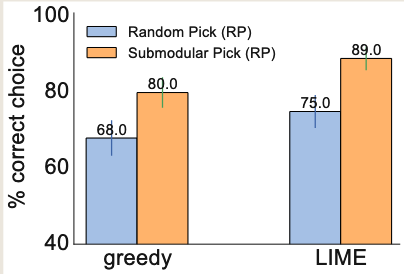
\includegraphics[width=0.6\textwidth]{img/img_9.png}
    \caption{人类受试者在两个分类器之间进行选择的平均准确率(有标准误差)。}
    \label{fig:img_9}
\end{figure}
\begin{figure}[h]
    \centering
    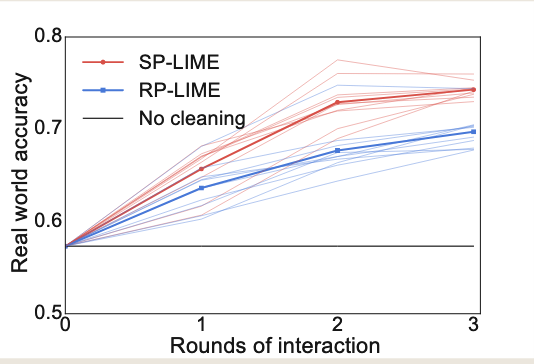
\includegraphics[width=0.6\textwidth]{img/img_10.png}
    \caption{特征工程实验。每条阴影线表示从初始 10 个主题之一开始的路径中主题的平均准确性。每条实线表示每轮交互中所有路径的平均值。}
    \label{fig:img_10}
\end{figure}
实验结果如图 9 所示。请注意,所有方法都能很好地识别出更好的分类器,这表明解释有助于确定应该信任哪个分类器,而使用测试集准确率则会导致选择错误的分类器。此外,我们还看到,与随机选择法(RP)相比,亚模块选择法(SP)大大提高了用户选择最佳分类器的能力,而 LIME 在这两种情况下的表现都优于贪婪法。
\subsection{非专家可以改进分类器吗?}
如果注意到分类器不可信,机器学习中的一个常见任务就是特征工程,即修改特征集和重新训练,以提高泛化能力。在这一过程中,解释可以通过呈现重要特征,尤其是移除用户认为不具有普遍性的特征来提供帮助。我们在这里也使用了 20 个新闻组数据,并要求 Amazon Mechanical Turk 用户为上一节(§6.2)中较差的分类器确定在后续训练中应删除解释中的哪些单词。在每一轮中,受试者在观察了 B = 10 个实例(每个解释中有 K = 10 个单词)后,会标记需要删除的单词(界面与图 2 类似,但使用的是单一算法)。需要提醒的是,这里的用户并不是机器学习方面的专家,也不熟悉特征工程,因此只能根据语义内容来识别词语。此外,用户无法访问宗教数据集,他们甚至不知道该数据集的存在。我们从 10 个受试者开始实验。在他们标记要删除的单词后,我们会训练 10 个不同的分类器,每个受试者一个(删除相应的单词)。然后,在新一轮互动中,每个分类器的解释会呈现给一组 5 个用户,从而产生 50 个新的分类器。最后一轮互动后,我们将得到 250 个分类器,每个分类器的互动路径都可以追溯到前 10 个主题。向每个用户展示的解释和实例由 SP-LIME 或 RP-LIME 生成。我们在图 10 中显示了宗教数据集在每一轮交互中,源自最初 10 个实验对象的路径的平均准确率(阴影线),以及所有路径的平均准确率(实线)。从图中可以明显看出,人群工作者能够通过去除他们认为对任务不重要的特征来改进模型。此外,SP-LIME 的表现优于 RP-LIME,这表明选择向用户展示的实例对于高效的特征工程至关重要。每个受试者每轮清理平均耗时 3.6 分钟,因此只用了不到 11 分钟就生成了分类器,该分类器对真实世界数据的泛化效果要好得多。使用 SP 时,每条路径平均删除了 200 个单词,而使用 RP 时则删除了 157 个单词,这表明将重要特征的覆盖范围纳入特征工程是非常有用的。此外,在 SP 算法平均选择的 200 个词中,至少有一半用户选择了 174 个词,而所有用户都选择了 68 个词。除了准确率的差异在各轮中都有所降低这一事实外,这种高度的一致性也表明用户正在向类似的正确模型靠拢。这项评估是一个例子,说明了如何通过解释来轻松改进不可信的分类器--在这种情况下,无需机器学习知识也能轻松改进。
\subsection{解释会带来见解吗?}
\begin{figure}[h]
    \centering
    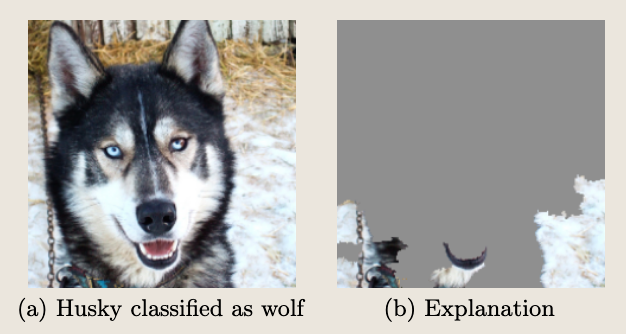
\includegraphics[width=0.6\textwidth]{img/img_11.png}
    \caption{“Husky vs Wolf ”任务中错误模型预测的原始数据和解释。}
    \label{fig:img_11}
\end{figure}
\begin{table}[h]
    \centering
    \caption{“Husky vs Wolf” 实验结果}
    \begin{tabular}{l c c}
    \toprule
     & Before & After \\
    \midrule
    Trusted the bad model & 10 out of 27 & 3 out of 27 \\
    Snow as a potential feature & 12 out of 27 & 25 out of 27 \\
    \bottomrule
    \end{tabular}
    \end{table}
数据收集过程中的人为因素往往会诱发分类器在训练过程中发现的不良相关性。这些问题很难通过查看原始数据和预测结果来识别。为了重现这样的环境,我们以区分狼和爱斯基摩犬(哈士奇)的照片为任务。我们在由 20 张图片组成的训练集上训练逻辑回归分类器,这些图片是人工挑选的,所有狼的照片背景都是雪,而哈士奇的照片背景不是雪。我们使用 Google 预先训练好的 Inception 神经网络[25]的第一个最大池化层作为图像特征。在另外 60 张图片上,如果有雪(或底部有浅色背景),分类器就会预测为 “狼”,否则就会预测为 “哈士奇”,而与动物的颜色、位置、姿势等无关。我们有意训练了这个糟糕的分类器,以评估受试者是否能够发现它。实验过程如下:我们首先给出一组均衡的 10 个测试预测(不含解释),其中一只狼不在雪地背景中(因此预测为 “哈士奇”),一只哈士奇在雪地背景中(因此预测为 “狼”)。图 11a 显示了 “哈士奇 ”的错误。其他 8 个例子都被正确分类。然后,我们向受试者提出三个问题:(1) 他们是否相信这种算法能在现实世界中很好地工作;(2) 为什么;(3) 他们认为该算法如何区分这些狼和哈士奇的照片。在得到这些回答后,我们展示带有相关解释的相同图片(如图 11b),并提出相同的问题。由于这项任务要求我们对虚假相关性和泛化的概念有一定的了解,因此本实验的受试者都是至少修过一门研究生机器学习课程的研究生。收集完回答后,我们让 3 位独立的评估者阅读他们的推理,并确定每位受试者是否提到了雪景、背景或同等条件作为模型可能使用的特征。我们选取大多数人的回答来判断受试者的见解是否正确,并在表 2 中报告了展示解释前后的这些数字。在观察解释之前,超过三分之一的受试者信任分类器,略少于一半的受试者提到神经网络正在使用雪的模式--尽管所有受试者都在猜测其他模式。然而,在观察了解释之后,几乎所有的受试者都指出了正确的见解,并且更加确定它是决定性因素。此外,受试者对分类器的信任度也大幅下降。虽然我们的样本量较小,但这个实验证明了解释个别预测对深入了解分类器的作用,知道何时不信任分类器以及为什么不信任。

\section{相关工作}
将验证集的准确性作为信任度的主要衡量标准所存在的问题已经得到了充分的研究。实践者总是高估模型的准确性[20],传播反馈回路[23],或者没有注意到数据泄露[14]。为了解决这些问题,研究人员提出了 Gestalt [21] 和 Modeltracker [1] 等工具,帮助用户浏览单个实例。在解释模型方面,这些工具是 LIME 的补充,因为它们并不解决解释单个预测的问题。此外,我们的子模态选取程序也可以纳入这些工具,帮助用户浏览更大的数据集。最近的一些工作旨在预测机器学习中的故障,特别是视觉任务[3, 29]。让用户知道系统何时可能出现故障,可以避免 “愚蠢的错误”,从而提高信任度[8]。这些解决方案要么需要额外的注释和专门针对视觉任务的特征工程,要么无法让用户深入了解为什么某个决策不可信。此外,它们还假设当前的评估指标是可靠的,但如果存在数据泄漏等问题,情况可能就不是这样了。最近的其他工作[11]侧重于让用户面对不同类型的错误(我们的选择步骤)。有趣的是,在他们的研究中,受试者即使看了很多错误,也没有注意到 20 个新闻组数据中的严重问题,这表明仅仅检查原始数据是不够的。需要注意的是,Groce 等人[11]在这方面并非孤例,该领域的许多研究人员都在不知不觉中发布了对这一任务不具普适性的分类器。通过使用 LIME,我们发现即使是非专家,也能在有解释的情况下识别出这些不规则现象。此外,LIME 还能补充现有系统的不足,让用户即使在预测看似 “正确 ”但却出于错误原因的情况下也能评估信任度。认识到解释在评估信任度中的作用,许多人建议使用可解释模型[27],尤其是在医疗领域[6, 17, 26]。虽然这些模型可能适用于某些领域,但未必同样适用于其他领域(例如,具有 5-10 个特征的超稀疏线性模型[26]不适合文本应用)。在这些情况下,可解释性是以灵活性、准确性或效率为代价的。对于文本而言,EluciDebug [16] 是一个完全的人在环系统,与我们的许多目标(可解释性、忠实性等)相同。不过,他们关注的是一个已经可以解释的模型(奈夫贝叶斯)。在计算机视觉领域,依靠物体检测产生候选排列[13]或注意力[28]的系统能够为其预测提供解释。然而,这些系统受限于特定的神经网络架构,或无法检测图像中的 “非物体 ”部分。在此,我们将重点放在通用的、与模型无关的解释上,这些解释可应用于任何适合该领域的分类器或回归器,甚至是尚未提出的分类器或回归器。模型无关解释的常见方法是在原始模型的预测上学习一个潜在的可解释模型[2, 7, 22]。将解释作为梯度向量[2],可以捕捉到与 LIME 类似的局部性直觉。然而,解释梯度上的系数是很困难的,特别是对于有把握的预测(梯度接近零)。此外,正如我们的实验所证明的那样,这些解释近似于原始模型的全局,因此保持局部保真度成为一项重大挑战。相比之下,LIME 解决的问题要可行得多,即找到一个能在局部逼近原始模型的模型。之前也有人探讨过扰动输入进行解释的想法[24],但与我们的通用框架不同,作者主要关注的是学习特定的贡献模型。这些方法都没有明确考虑认知的局限性,因此可能会产生不可解释的解释,如梯度或具有数千个非零权重的线性模型。如果原始特征对人类来说毫无意义(如单词嵌入),问题就会变得更加严重。相比之下,LIME 将可解释性纳入优化和可解释表征的概念中,这样就能满足特定领域和任务的可解释性标准。
\section {结论和未来工作}
在本文中,我们认为信任对于人类与机器学习系统的有效互动至关重要,而解释个体预测对于评估信任度非常重要。我们提出了 LIME,这是一种模块化、可扩展的方法,能以可解释的方式忠实地解释任何模型的预测。我们还引入了 SP-LIME,这是一种选择代表性和非冗余预测的方法,可为用户提供模型的全局视图。我们的实验表明,在文本和图像领域与信任相关的任务中,解释对各种模型都很有用,专家和非专家用户都可以使用:在不同模型之间做出决定、评估信任度、改进不可信的模型,以及深入了解预测结果。我们希望在未来的工作中探索一些途径。虽然我们只将稀疏线性模型描述为解释,但我们的框架支持对决策树等各种解释系列进行探索;如果能与真实用户一起对这些解释进行比较研究,将会非常有趣。我们在这项工作中没有提到的一个问题是如何执行图像的挑选步骤,我们希望在未来解决这一局限性。领域和模型无关性使我们能够探索各种应用,我们希望研究在语音、视频和医疗领域以及推荐系统中的潜在应用。最后,我们希望探索理论特性(如适当的样本数量)和计算优化(如使用并行化和 GPU 处理),以便提供准确、实时的解释,这对任何人在环机器学习系统都至关重要。
\end{document}
